\documentclass[fleqn,12pt]{article}

\usepackage[utf8]{inputenc}
\usepackage[T1]{fontenc}
\usepackage{mathtools} %loads amsmath
\usepackage{amsthm}
\usepackage{amsfonts}
\usepackage{amsmath}
\usepackage{amssymb}
\usepackage{graphicx}
\usepackage{tikz}
\usetikzlibrary{arrows,automata,positioning}
\usepackage{arydshln}
\usepackage{stmaryrd}
\usepackage{pdflscape}

\tikzset{initial text={}}

\usepackage{fancyhdr}
\setlength{\headheight}{26pt}
\pagestyle{fancy}
\lhead{Static Program Analysis WS 2016/17 -- Series 06 \\ \small{Igor Dudschenko (296764), Oliver Westphal (358321)}}
\rhead{}

\newcommand\dbrackets[1]{\llbracket #1 \rrbracket}

\setlength{\parindent}{0cm}
\newcommand\note[1]{\textcolor{red}{#1}}

\begin{document}
\section*{Exercise 1}
\subsection*{a)}
\begin{tikzpicture}[node distance = 0.33cm]
   \node[state,initial,rectangle] (1)   {$[x := -1;]^1$}; 
   \node[state,rectangle] (2) [below=of 1] {$[y:=-2*x;]^2$}; 
   \node[state,rectangle] (3) [below =of 2] {$while[(y-1>x)]^3$}; 
   \node[state,rectangle](4) [below =of 3] {$[assert (y-1>x)]^4$};
   \node[state,rectangle](5) [below =of 4] {$[y:=y-1]^5$};
   \node[state,rectangle](6) [below =of 5] {$if[x>-2]^6$};
   \node[state,rectangle](7) [below =of 6] {$[assert (x>-2)]^7$};
   \node[state,rectangle](8) [below =of 7] {$[x:=x-1]^8$};
   \node[state,rectangle](9) [right=of 6] {$[assert (x \leq -2)]^9$};
   \node[state,rectangle](10) [right =of 3] {$[assert (y-1 \leq x)]^{10}$};
   \node[state,rectangle](11) [below =of 10] {$[skip]^{11}$};   
    \path[->] (1) edge  node {} (2);
    \path[->] (2) edge  node {} (3);
    \path[->] (3) edge  node {} (4);
    \path[->] (4) edge  node {} (5);
    \path[->] (5) edge  node {} (6);
    \path[->] (6) edge  node {} (7);
    \path[->] (7) edge  node {} (8);
    \path[->] (3) edge  node {} (10);
    \path[->] (10) edge  node {} (11);
    \path[->] (6) edge  node {} (9);
    \draw [->, bend angle=35, bend right] (9) to (3);
    \draw [->, bend angle=75, bend left] (8) to (3);
\end{tikzpicture}
\begin{landscape}
\subsection*{b)}
\begin{tabular}{c|c|c|c|c|c|c|c|c|c|c|c}
Worklist & $Al_1$ & $Al_2$ & $Al_3$ & $Al_4$ & $Al_5$ & $Al_6$ & $Al_7$ & $Al_8$ & $Al_9$ & $Al_{10}$ & $Al_{11}$\\
\hline
12,23,34,45,56,67,78,69,93,3 10,10 11 & $[-\infty,+\infty]$ & $\emptyset$ & $\emptyset$ & $\emptyset$ & $\emptyset$ & $\emptyset$ & $\emptyset$ & $\emptyset$ & $\emptyset$ & $\emptyset$ & $\emptyset$\\
\end{tabular}
\end{landscape}
\subsection*{c)}
\section*{Exercise 2}
\section*{Exercise 3}
\subsection*{a)}
Use $(D,\sqsubseteq)$ with\\
$D := (Lab_c \cup \top)^{\leq m_s} \cup \{\text{None, Error}\}$ where $l \in Lab_c$ represent uninitialized values created at label $l$. To make this clear we write $\bot^l$ instead of just $l$.\\

for every $S=\sigma_1\dots\sigma_n \in D$, $\text{None} \sqsubseteq S$ and $S \sqsubseteq \text{Error}$\\
$S \sqsubseteq S'$ iff $S=\sigma_1\dots\sigma_n$ $S'=\sigma_1'\dots\sigma_n'$ and $\sigma_i \sqsubseteq_{def} \sigma_i'$\\
$\sqsubseteq_{def}$ is defined as $s \sqsubseteq s$ and $\top \sqsubseteq s$ for all $s \in Lab_c \cup \top$.
\subsection*{b)}
Let $l \in Lab_c$ denote the label of the respective instruction\\

new C: $S \rightarrow \bot^l.S$ if $|S| < m_s$\\
iconst z: $S \rightarrow \top.S$ if $|S| < m_s$\\
aconst null: $S \rightarrow \bot^l.S$ if $|S| < m_s$\\
if\_cmpeq l: $x.y.S \rightarrow S$ if $|S| < m_s$\\
aload n: $S \rightarrow \top.S$ if $0\leq n < m_r, |S| < m_s$\\
astore n: $\top.S \rightarrow S$ if $0\leq n < m_r$\\
getfield C f $\tau$: $\top.S \rightarrow \top.S$ if $|S| < m_s$\\
putfield C f $\tau$: $\top.\top.S \rightarrow \top.S$ if $|S| < m_s$ \\
invoke C M $\sigma$: $\underbrace{\top\dots\top}_{n-times}.\top.S \rightarrow \top.S$ if $\sigma = \tau_0(\tau_1,\dots,\tau_n),|S| < m_s$\\
invokespecial C M $\sigma$: $\underbrace{\top\dots\top}_{n-times}.\bot^l.S \rightarrow S\underbrace{[\bot^l \rightarrow \top]}_{\text{substitution}}$ 
\begin{flushright}
if $\sigma = (\tau_1,\dots,\tau_n)$ and $B^l =$ new C
\end{flushright}
dup: $x.S \rightarrow x.x.S$ if $x \in Lab_c \cup \top, |x.S| < m_s$\\
\subsection*{c)}
Worklist: $W = \{ (1,2),(2,3),(3,4),(4,5),(5,6),(5,9),(6,7),(7,8),$\\
$(8,14),(9,10),(10,11),(11,12),(12,13),(13,14) \}$ (no cyclic dependencies).
Extremal value: $\iota = \epsilon$ (assume empty stack in the beginning)\\

\begin{tabular}{c|c|c}
Label & Instruction & S \\ 
\hline 
1 & new A & $\epsilon$ \\ 
2 & dup & None $\overset{(1,2)}{\rightarrow} \bot^1$ \\ 
3 & aload 1 & None $\overset{(2,3)}{\rightarrow} \bot^1.\bot^1$ \\ 
4 & aconst null & None $\overset{(3,4)}{\rightarrow} \top.\bot^1.\bot^1$\\ 
5 & if\_cmpeq 9 & None $\overset{(4,5)}{\rightarrow} \bot^4.\top.\bot^1.\bot^1$\\ 
6 & aload 1 & None $\overset{(5,6)}{\rightarrow} \bot^1.\bot^1$ \\ 
7 & invokespezial A <init> (B) & None $\overset{(6,7)}{\rightarrow} \top.\bot^1.\bot^1$ \\ 
8 & goto 14 & None $\overset{(7,8)}{\rightarrow} \top$\\  
9 & new B & None $\overset{(5,9)}{\rightarrow} \bot^1.\bot^1$\\  
10 & dup & None $\overset{(9,10,)}{\rightarrow} \bot^9.\bot^1.\bot^1$\\  
11 & iconst 3 & None $\overset{(10,11)}{\rightarrow} \bot^9.\bot^9.\bot^1.\bot^1 $\\ 
12 & invokespezial B <init> (A,int) & None $\overset{(11,12)}{\rightarrow} \top.\bot^9.\bot^9.\bot^1.\bot^1 $\\  
13 & invokespezial A <init> (B) & None $\overset{(12,13)}{\rightarrow} \text{Error}$\\  
14 & astore 0 & None $\overset{(8,14)}{\rightarrow} \top \overset{(13,14)}{\rightarrow} \top \sqcup \text{Error} = \text{Error}$\\ 
\end{tabular} 
\end{document}
